%  A simple AAU report template.
%  2015-05-08 v. 1.2.0
%  Copyright 2010-2015 by Jesper Kjær Nielsen <jkn@es.aau.dk>
%
%  This is free software: you can redistribute it and/or modify
%  it under the terms of the GNU General Public License as published by
%  the Free Software Foundation, either version 3 of the License, or
%  (at your option) any later version.
%
%  This is distributed in the hope that it will be useful,
%  but WITHOUT ANY WARRANTY; without even the implied warranty of
%  MERCHANTABILITY or FITNESS FOR A PARTICULAR PURPOSE.  See the
%  GNU General Public License for more details.
%
%  You can find the GNU General Public License at <http://www.gnu.org/licenses/>.
%
%  A simple AAU report template.
%  2015-05-08 v. 1.2.0
%  Copyright 2010-2015 by Jesper Kjær Nielsen <jkn@es.aau.dk>
%
%  This is free software: you can redistribute it and/or modify
%  it under the terms of the GNU General Public License as published by
%  the Free Software Foundation, either version 3 of the License, or
%  (at your option) any later version.
%
%  This is distributed in the hope that it will be useful,
%  but WITHOUT ANY WARRANTY; without even the implied warranty of
%  MERCHANTABILITY or FITNESS FOR A PARTICULAR PURPOSE.  See the
%  GNU General Public License for more details.
%
%  You can find the GNU General Public License at <http://www.gnu.org/licenses/>.
%
\documentclass[11pt,twoside,a4paper,openright]{report}
%%%%%%%%%%%%%%%%%%%%%%%%%%%%%%%%%%%%%%%%%%%%%%%%
% Language, Encoding and Fonts
% http://en.wikibooks.org/wiki/LaTeX/Internationalization
%%%%%%%%%%%%%%%%%%%%%%%%%%%%%%%%%%%%%%%%%%%%%%%%
% Select encoding of your inputs. Depends on
% your operating system and its default input
% encoding. Typically, you should use
%   Linux  : utf8 (most modern Linux distributions)
%            latin1 
%   Windows: ansinew
%            latin1 (works in most cases)
%   Mac    : applemac
% Notice that you can manually change the input
% encoding of your files by selecting "save as"
% an select the desired input encoding. 
\usepackage[utf8]{inputenc}
% Make latex understand and use the typographic
% rules of the language used in the document.
\usepackage[danish]{babel}
% Use the palatino font
\usepackage[sc]{mathpazo}
\linespread{1.05}         % Palatino needs more leading (space between lines)
% Choose the font encoding
\usepackage[T1]{fontenc}
%%%%%%%%%%%%%%%%%%%%%%%%%%%%%%%%%%%%%%%%%%%%%%%%
% Graphics and Tables
% http://en.wikibooks.org/wiki/LaTeX/Importing_Graphics
% http://en.wikibooks.org/wiki/LaTeX/Tables
% http://en.wikibooks.org/wiki/LaTeX/Colors
%%%%%%%%%%%%%%%%%%%%%%%%%%%%%%%%%%%%%%%%%%%%%%%%
% load a colour package
\usepackage{xcolor}
\definecolor{aaublue}{RGB}{33,26,82}% dark blue
% The standard graphics inclusion package
\usepackage{graphicx}
\graphicspath{{./grafik/}}
% Set up how figure and table captions are displayed
\usepackage{caption}
\captionsetup{%
  font=footnotesize,% set font size to footnotesize
  labelfont=bf % bold label (e.g., Figure 3.2) font
}
\usepackage{pdfpages}
\usepackage[numbers, sort&compress]{natbib}
% Make the standard latex tables look so much better
\usepackage{array,booktabs}
% Enable the use of frames around, e.g., theorems
% The framed package is used in the example environment
\usepackage{framed}
\usepackage[linewidth=2pt]{mdframed} %Bliver brugt til at lave en ramme om ting

%%%%%%%%%%%%%%%%%%%%%%%%%%%%%%%%%%%%%%%%%%%%%%%%
% Mathematics
% http://en.wikibooks.org/wiki/LaTeX/Mathematics
%%%%%%%%%%%%%%%%%%%%%%%%%%%%%%%%%%%%%%%%%%%%%%%%
% Defines new environments such as equation,
% align and split 
\usepackage{amsmath}
% Adds new math symbols
\usepackage{amssymb}
% Use theorems in your document
% The ntheorem package is also used for the example environment
% When using thmmarks, amsmath must be an option as well. Otherwise \eqref doesn't work anymore.
\usepackage[framed,amsmath,thmmarks]{ntheorem}

%%%%%%%%%%%%%%%%%%%%%%%%%%%%%%%%%%%%%%%%%%%%%%%%
% Page Layout
% http://en.wikibooks.org/wiki/LaTeX/Page_Layout
%%%%%%%%%%%%%%%%%%%%%%%%%%%%%%%%%%%%%%%%%%%%%%%%
% Change margins, papersize, etc of the document
\usepackage[
  inner=28mm,% left margin on an odd page
  outer=41mm,% right margin on an odd page
  ]{geometry}
% Modify how \chapter, \section, etc. look
% The titlesec package is very configureable
\usepackage{titlesec}
\titleformat{\chapter}[display]{\normalfont\huge\bfseries}{\chaptertitlename\ \thechapter}{20pt}{\Huge}
\titleformat*{\section}{\normalfont\Large\bfseries}
\titleformat*{\subsection}{\normalfont\large\bfseries}
\titleformat*{\subsubsection}{\normalfont\normalsize\bfseries}
%\titleformat*{\paragraph}{\normalfont\normalsize\bfseries}
%\titleformat*{\subparagraph}{\normalfont\normalsize\bfseries}

% Clear empty pages between chapters
\let\origdoublepage\cleardoublepage
\newcommand{\clearemptydoublepage}{%
  \clearpage
  {\pagestyle{empty}\origdoublepage}%
}
\let\cleardoublepage\clearemptydoublepage

% Change the headers and footers
\usepackage{fancyhdr}
\pagestyle{fancy}
\fancyhf{} %delete everything
\renewcommand{\headrulewidth}{0pt} %remove the horizontal line in the header
\fancyhead[RE]{\small\nouppercase\leftmark} %even page - chapter title
\fancyhead[LO]{\small\nouppercase\rightmark} %uneven page - section title
\fancyhead[LE,RO]{\thepage} %page number on all pages
% Do not stretch the content of a page. Instead,
% insert white space at the bottom of the page
\raggedbottom
% Enable arithmetics with length. Useful when
% typesetting the layout.
\usepackage{calc}

%%%%%%%%%%%%%%%%%%%%%%%%%%%%%%%%%%%%%%%%%%%%%%%%
% Bibliography
% http://en.wikibooks.org/wiki/LaTeX/Bibliography_Management
%%%%%%%%%%%%%%%%%%%%%%%%%%%%%%%%%%%%%%%%%%%%%%%%
%\usepackage[backend=bibtex,
%  bibencoding=utf8
%  ]{biblatex}
%\addbibresource{bib}

%%%%%%%%%%%%%%%%%%%%%%%%%%%%%%%%%%%%%%%%%%%%%%%%
% Misc
%%%%%%%%%%%%%%%%%%%%%%%%%%%%%%%%%%%%%%%%%%%%%%%%
% Add bibliography and index to the table of
% contents
\usepackage[nottoc]{tocbibind}
% Add the command \pageref{LastPage} which refers to the
% page number of the last page
\usepackage{lastpage}
% Add todo notes in the margin of the document
\usepackage[
%  disable, %turn off todonotes
  colorinlistoftodos, %enable a coloured square in the list of todos
  textwidth=\marginparwidth, %set the width of the todonotes
  textsize=scriptsize, %size of the text in the todonotes
  ]{todonotes}

%%%%%%%%%%%%%%%%%%%%%%%%%%%%%%%%%%%%%%%%%%%%%%%%
% Hyperlinks
% http://en.wikibooks.org/wiki/LaTeX/Hyperlinks
%%%%%%%%%%%%%%%%%%%%%%%%%%%%%%%%%%%%%%%%%%%%%%%%
% Enable hyperlinks and insert info into the pdf
% file. Hypperref should be loaded as one of the 
% last packages
\usepackage{hyperref}
\hypersetup{%
	pdfpagelabels=true,%
	plainpages=false,%
	pdfauthor={Author(s)},%
	pdftitle={Title},%
	pdfsubject={Subject},%
	bookmarksnumbered=true,%
	colorlinks=true,%
	citecolor=black,%
	filecolor=black,%
	linkcolor=black,% you should probably change this to black before printing
	urlcolor=black,%
	pdfstartview=FitH%
}

\usepackage{enumitem}
\usepackage{caption}
\usepackage{subcaption}
\usepackage[danish,nameinlink,capitalise]{cleveref}
\usepackage{listings}

\usepackage{tikz}
\usetikzlibrary{arrows}

% Additional commands
\newcommand{\namedtodo}[5]
{
  \ifthenelse{\equal{#1}{}}
  {
    \todo[backgroundcolor=#4,caption=
    {\textbf{#3: } #2}
    ,inline]
    {\color{#5}\textbf{#3: }#2}
  }
  {
    \todo[backgroundcolor=#4,caption=
    {\textbf{#3: } #1}
    ,inline]
    {\color{#5}\textbf{#3: }#2}
  }
}
\newcommand{\mikkel}[2][]{\namedtodo{#1}{#2}{Mikkel}{blue!80}{white}}
\newcommand{\stefan}[2][]{\namedtodo{#1}{#2}{Stefan M}{orange}{black}}
\newcommand{\mikael}[2][]{\namedtodo{#1}{#2}{Mikael}{green}{black}}
\newcommand{\bruno}[2][]{\namedtodo{#1}{#2}{Bruno}{black!10!red!90}{white}}
\newcommand{\lasse}[2][]{\namedtodo{#1}{#2}{Lasse}{black!10!yellow!90}{black}}
\newcommand{\als}[2][]{\namedtodo{#1}{#2}{Als}{purple!90!orange}{white}}
\newcommand{\winde}[2][]{\namedtodo{#1}{#2}{Winde}{black}{white}}
\newcommand{\lars}[2][]{\namedtodo{#1}{#2}{Lars}{blue!80}{black}}
\newcommand{\ivan}[2][]{\namedtodo{#1}{#2}{Ivan}{red}{black}}


  \makeatletter \renewcommand \listoftodos{\section*{List of Todos} \@starttoc{tdo}}
  \renewcommand\l@todo[2]
    {\par\noindent \textit{#2}, \parbox{10cm}{#1}\par} \makeatother
% Her er en liste over navnene på de forskellige styles
% C#: csharp
% F#: fsharp

% 
% Listings kan refereres vha. \cref{}
\crefname{listing}{code example}{code example}
\Crefname{listing}{Code example}{code examples}
% 

%Algoritmer i cref
\crefname{algocf}{algorithm}{algorithm}
\Crefname{algocf}{Algorithm}{Algorithms}
%Algoritmelinjer i cref
\crefalias{AlgoLine}{line}%

\makeatletter
\let\cref@old@stepcounter\stepcounter
\def\stepcounter#1{%
  \cref@old@stepcounter{#1}%
  \cref@constructprefix{#1}{\cref@result}%
  \@ifundefined{cref@#1@alias}%
    {\def\@tempa{#1}}%
    {\def\@tempa{\csname cref@#1@alias\endcsname}}%
  \protected@edef\cref@currentlabel{%
    [\@tempa][\arabic{#1}][\cref@result]%
    \csname p@#1\endcsname\csname the#1\endcsname}}
\makeatother
%

% Angivelse af navn på listings
\renewcommand\lstlistingname{Code example}
\renewcommand\lstlistlistingname{Code example}

\lstdefinestyle{standard}
{
	frame=shadowbox,
	framesep=5pt,
	rulecolor=\color{blue!40!black},
	rulesepcolor=\color{white!93!black},
	numbers=left,
	basicstyle=\ttfamily,
	numberstyle=\tiny,
	numberfirstline=true,
	%numberblanklines=false,
	stepnumber=1,
	numbersep=9pt,	
	captionpos=b,
	escapeinside={(*}{*)},
	breaklines=true,
	tabsize=4,
	language=c
}

\lstset{style=standard}

\lstdefinestyle{c}
{
	style=standard
}

\lstdefinestyle{csmall}
{
	style=c
}

\lstdefinestyle{csharp}
{
	style=standard,
	language=[Sharp]C
}
\lstdefinestyle{csharpsmall}
{
	style=csharp
}
\lstdefinestyle{fsharp}
{
	language=[Sharp]F,
	frame=lr,
	rulecolor=\color{blue!80!black}
}
\lstdefinestyle{fsharpsmall}
{
	style=fsharp,
	basicstyle=\ttfamily\footnotesize
}


% Definitions

% Superscript and subscript
\newcommand{\superscript}[1]{\ensuremath{^{\textrm{#1}}}}
\newcommand{\subscript}[1]{\ensuremath{_{\textrm{#1}}}}

% Degrees
\newcommand{\degree}{\ensuremath{^\circ}}
\newcommand{\dg}{\degree}

\newcommand{\quoter}[1]%
{
  \par
  \vspace{1.5em}
  \addtolength{\leftskip}{1.5cm}
  \addtolength{\rightskip}{1.5cm}
  \textit{#1}
  \addtolength{\leftskip}{-1.5cm}
  \addtolength{\rightskip}{-1.5cm}
  \vspace{1.5em}
  \par
}


\newcommand{\sensor}[3]
{
	\section{#1}
	#2
	
	#3
}

\newcommand{\analyse}[2]
{
\subsection{#1}
#2
}


% package inclusion and set up of the document
% see, e.g., http://en.wikibooks.org/wiki/LaTeX/Formatting#Hyphenation
% for more information on word hyphenation
\hyphenation{ex-am-ple hy-phen-a-tion short}
\hyphenation{long la-tex}
% 
%  A simple AAU report template.
%  2015-05-08 v. 1.2.0
%  Copyright 2010-2015 by Jesper Kjær Nielsen <jkn@es.aau.dk>
%
%  This is free software: you can redistribute it and/or modify
%  it under the terms of the GNU General Public License as published by
%  the Free Software Foundation, either version 3 of the License, or
%  (at your option) any later version.
%
%  This is distributed in the hope that it will be useful,
%  but WITHOUT ANY WARRANTY; without even the implied warranty of
%  MERCHANTABILITY or FITNESS FOR A PARTICULAR PURPOSE.  See the
%  GNU General Public License for more details.
%
%  You can find the GNU General Public License at <http://www.gnu.org/licenses/>.
%
%
%
% see, e.g., http://en.wikibooks.org/wiki/LaTeX/Customizing_LaTeX#New_commands
% for more information on how to create macros

%%%%%%%%%%%%%%%%%%%%%%%%%%%%%%%%%%%%%%%%%%%%%%%%
% Macros for the titlepage
%%%%%%%%%%%%%%%%%%%%%%%%%%%%%%%%%%%%%%%%%%%%%%%%
%Creates the aau titlepage
\newcommand{\aautitlepage}[3]{%
  {
    %set up various length
    \ifx\titlepageleftcolumnwidth\undefined
      \newlength{\titlepageleftcolumnwidth}
      \newlength{\titlepagerightcolumnwidth}
    \fi
    \setlength{\titlepageleftcolumnwidth}{0.5\textwidth-\tabcolsep}
    \setlength{\titlepagerightcolumnwidth}{\textwidth-2\tabcolsep-\titlepageleftcolumnwidth}
    %create title page
    \thispagestyle{empty}
    \noindent%
    \begin{tabular}{@{}ll@{}}
      \parbox{\titlepageleftcolumnwidth}{
        \iflanguage{danish}{%
          \includegraphics[width=.8\titlepageleftcolumnwidth]{aau_logo_da}
        }{%
          \includegraphics[width=.8\titlepageleftcolumnwidth]{aau_logo_en}
        }
      } &
      \parbox{\titlepagerightcolumnwidth}{\raggedleft\sf\small
        #2
      }\bigskip\\
       #1 &
      \parbox[t]{\titlepagerightcolumnwidth}{%
      \textbf{Abstract:}\bigskip\par
        \fbox{\parbox{\titlepagerightcolumnwidth-2\fboxsep-2\fboxrule}{%
          #3
        }}
      }\\
    \end{tabular}
    \vfill
    \iflanguage{danish}{%
      \noindent{\footnotesize\emph{Rapportens indhold er frit tilgængeligt, men offentliggørelse (med kildeangivelse) må kun ske efter aftale med forfatterne.}}
    }{%
      \noindent{\footnotesize\emph{The content of this report is freely available, but publication (with reference) may only be pursued due to agreement with the author.}}
    }
    \clearpage
  }
}

%Create english project info
\newcommand{\englishprojectinfo}[8]{%
  \parbox[t]{\titlepageleftcolumnwidth}{
    \textbf{Title:}\\ #1\bigskip\par
    \textbf{Theme:}\\ #2\bigskip\par
    \textbf{Project Period:}\\ #3\bigskip\par
    \textbf{Project Group:}\\ #4\bigskip\par
    \textbf{Participant(s):}\\ #5\bigskip\par
    \textbf{Supervisor(s):}\\ #6\bigskip\par
    \textbf{Copies:} #7\bigskip\par
    \textbf{Page Numbers:} \pageref{LastPage}\bigskip\par
    \textbf{Date of Completion:}\\ #8
  }
}

%Create danish project info
\newcommand{\danishprojectinfo}[8]{%
  \parbox[t]{\titlepageleftcolumnwidth}{
    \textbf{Titel:}\\ #1\medskip \par
    \textbf{Tema:}\\ #2\medskip \par
    \textbf{Projektperiode:}\\ #3\medskip \par
    \textbf{Projektgruppe:}\\ #4\medskip \par
    \textbf{Deltager(e):}\\ #5\medskip \par
    \textbf{Vejleder(e):}\\ #6\medskip \par
    \textbf{Oplagstal:} #7\medskip \par
    \textbf{Sidetal:} \pageref{LastPage}\medskip \par
    \textbf{Afleveringsdato:}\\ #8
  }
}

%%%%%%%%%%%%%%%%%%%%%%%%%%%%%%%%%%%%%%%%%%%%%%%%
% An example environment
%%%%%%%%%%%%%%%%%%%%%%%%%%%%%%%%%%%%%%%%%%%%%%%%
\theoremheaderfont{\normalfont\bfseries}
\theorembodyfont{\normalfont}
\theoremstyle{break}
\def\theoremframecommand{{\color{gray!50}\vrule width 5pt \hspace{5pt}}}
%\newshadedtheorem{exa}{Example}[chapter]
%\newenvironment{example}[1]{%
%		\begin{exa}[#1]
%}{%
%		\end{exa}
%}
% my new macros


\begin{document}
\pagestyle{empty} %disable headers and footers
\pagenumbering{roman} %use roman page numbering in the frontmatter


\pagestyle{fancy} %enable headers and footers again
\setcounter{tocdepth}{1}
\listoftodos
%\input{sections/preface.tex}
%mainmatter
\pagenumbering{arabic} %use arabic page numbering in the mainmatter

\section{Relationen mellem projekt og de fire varianter}
%A relation of your project to software innovation variants (see Essence-book Section 5.1).
Dette afsnit beskriver relationen mellem de fire varianter af software innovation\cite[Afsnit 5.1, Side 30-32]{art:essence} og PsyLog projektet.
Hertil gives først en kort gennemgang af hvilke af de fire varianter der relaterer sig til projektet.
Dernæst beskrives det, for disse varianter, i yderligere detalje hvordan denne relation kommer til udtryk.

\paragraph{Relaterbare innovations varianter}
Eftersom PsyLog repræsenterer en ny tilgang til indsamling af patientinformation, anses \textit{proces innovation} som den af de fire varianter der bedst relaterer sig til PsyLog projektet.

\textit{Projekt innovation} relaterer sig ligeledes til den overordnede problemstilling, men beskriver ikke i samme omfang det syn på innovation projektgruppens medlemmer deler.

\textit{Produkt innovation} relaterer sig ikke så godt til PsyLog, da projektet sigter mod etablering af en platform og på den måde ikke et produkt i en klassisk forstand.
I stedet ses platformen som en mulighed for udvikling af diverse moduler.
Kombinationen af moduler anses som produkter.
Dermed kan den overordnede platform anses som en mulighed for udvikling af en række produkter, men ikke et produkt i sig selv.

\textit{Paradigme innovation} relaterer sig ligeledes til PsyLog.
Denne relation minder om relationen til process innovation, men ikke lige så direkte.
Dette detaljeres yderligere herunder.

%\subsection{Produkt innovation}
% Product innovation is about developing new or improved software-intensive products.

\subsection{Proces innovation}
% Process Innovation is about developing software-intensive solutions that offer users new or improved ways to produce their existing products or services.
Indsamling af information om personlig adfærd hos en patient foretages pt ved at patienten løbende tager noter om adfærd eller ved at foretage interviews.
Noterne kan anvendes til personlig refleksion mens interviews vil give en psykolog eller psykiater mulighed for at klarlægge patientens normale adfærd.
Med en af disse typer information bliver det muligt at registrere ændringer i adfærd.
Dog er begge typer information påvirket af patientens subjektive vurdering.

Hertil kan et system som PsyLog anvendes til at indsamle information om patientens adfærd.
Herved opnås to forbedringer på ovenstående proces.
For det første vil information indsamles kontinuert og uafhængigt af kontekst.
Altså indsamles information ikke kun i situationer hvor patienten ønsker at notere dette eller i forbindelse med forudplanlagte interviews.
Derudover fjernes brugerens subjektive påvirkning af informationer og der skabes derved et mere objektivt billede af patientens egentlige adfærd.

\subsection{Projekt innovation}
% Project innovation is when existing software solutions are fitted into new application domains (illustrated in Section 4.3) – what Tidd et al. labels position innovation.
Der findes flere forskellige eksisterende applikationer der monitorerer adfærd ved hjælp af en mobiltelefon.
Der findes eksempelvis applikationer der indsamler information om rute og hastighed i forbindelse med løbe- eller cykelture.
Tilsvarende findes også applikationer der monitorerer søvnmønstre og ud fra dette angiver hvornår brugeren skal vækkes.

Applikationer som disse vil kunne anvendes til at detektere ændringer i adfærd, hvilket kan anvendes som indikator på ændring i en patients stemningsleje.
Dog bemærkes det at disse applikationer samler information om meget specifikke problemområder.
For at kunne anvende disse informationer, vil det derfor være nødvendigt at trække information ud fra en række eksisterende applikationer, for derefter at kombinere dem i en sideløbende applikation.

\subsection{Paradigme innovation}
% Finally, Paradigm innovation is when software-intensive solutions are coupled with changes in the ‘mental models’ which frame what an organization is about; who the users are; or what the market is or wants (illustrated in Section 4.1).
Endeligt relaterer paradigme innovation sig til PsyLog ved at ændre tankegangen om hvordan adfærd registreres.
Da informationer om patienten kun leveres af patienten selv, beskriver den eksisterende mentale model indsamlinger af informationer om patienten som noget privat og personligt.
Ved anvendelse af PsyLog bliver disse private informationer indsamlet af et autonomt system.
Således sker der et skift i modellen, ved at fjerne det filter patienten bevidst eller ubevidst påfører dataindsamlingen.

Herved relaterer paradigme innovation sig ikke lige så direkte til PsyLog som process innovation, men beskriver i store træk den samme innovation.
Derved vurderer projektgruppens medlemmer at paradigme innovation ikke relaterer sig godt til PsyLog projektet.

\section{VBM review}
For at give et eksempel på et VBM review beskrives vores vision inquiry review.
Vores vision inquiry baserer sig på teorien beskrevet i \citet[afsnit 10.5, side 66]{art:essence}.
At foretage dette review sikrer at visionen giver en beskrivelse af relationen mellem problem og løsning der er rammende.
Dermed ikke sagt at visionen skal give en udtømmende beskrivelse, men rettere at give en forståelse af hvad hovedidéerne er ved projektet.

Visionen der foretages et Vision Inquiry på er fra konfigurationstabellen der kan ses i \cref{tab:konfigurationsTabel}.
Vision Inquiry   F-16
\begin{description}[style=nextline]
	\item[Is the Vision brief and communicable?]
		Visionen om F-16 er kortfattet. 
		Dog kan der herske forvirring da man kan forestille sig død og ødelæggelse i stedet for modularitet der menes.
		Dog understøttes denne vision af andre metaforer og en proposition, hvorfor dette ikke regnes for et problem.
	\item[Does the Vision aptly link solution to problem?]
		Visionen passer godt på løsningen, da løsningen er modulær ligesom F-16 flyet.
	\item[Are the Grounds related to the Use context?]
		Nej, de er ikke relaterede da use context snakker om teknologi hvor Grounds snakker om affektive lidelser.
	    Der mangler altså et bindeled mellem hvad teknologien har med affektive lidelser at gøre.
	    En mulig omformulering kunne være at omformulere grounds til "depressions- og mani-perioder opdages for sent, men kan opdages vha. data fra smartphones".
	\item[Does the Warrant provide good reason to solve the problem?]
		Ja, det er en meget god grund til at løse problemet.
	\item[Does the Qualifier identify key limitations relative to the Challenge?]
		Den siger man skal have en basal viden om smartphones.
		Begrænsning i forhold til teori om registrering af adfærdsændringer nævnes ikke.
	\item[Does the Rebuttal recognize the solution as acceptable?]
		Ja, det er meget god grund, da man kan reducere antallet af behandlinger, og dermed omkostninger på dette felt.
	\item[Does the features offer a sound idea about how the solution solves the problem?]
		Features giver ikke en særlig god ide om hvordan de løser problemet.
		Savner bedre beskrivelse af interne features.
\end{description}

Findings fundet er derefter input til den næste sprint planning aktivitet, og dette kan også føre til ændringer i visionen. 

\chapter{Essence}
I dette afsnit bliver diverse Essence emner præsenteret og detaljeret.
\section{Beskrivelse af problem}


\section{Tidlig konfigurationstabel}
En konfiguration af et system er en kombination af elementer, og en konfigurationstabel beskriver den konfiguration.

Denne beskrivelse er baseret på  \citet[Afsnit 3.2, Side 16-21]{art:essence}.

Systemets `use context' er at systemet bruges til at informere unipolare og bipolare patienter om der har været åbenbare adfærdsændringer. Udfordringen er så om mobilen kan bruges til at gøre dette ved hjælp af sensorer på mobilen.

Den øverste række i \cref{tidlig_konfigurationstabel} navngiver de fire Views i Essence: Paradigm, Product, Project og Process.

`Focus' rækken repræsenterer de største problemer og løsninger i projektet. 
Udfordringen er tiltænkt til at være om man kan bruge en mobil til at overvåge adfærd af psykisk syge og se om den ændrer sig. 
Use context er så tiltænkt at de psykiske syge bruger deres mobil i deres hjem og andre vante omgivelser. 
Så er det tiltænkt at product affordance er at adfærdsdata bruges til at estimere patientens sindstilstand, med den mulighed at denne data kan deles med andre som kan bruge denne data til at hjælpe behandlingen. 
Løsnings strategien er så at bruge en smartphone, og udvikle et system som kan registrere data fra forskellige sensorer for at kompensere for subjektive data der vides om sygdomsforløbet..
Data den indsamler skal være objektiv, så idéen er at den skal fungere som en objektiv dagbog, eller som en fitness tracker der i stedet for at spore fysisk helbred ser på psykisk helbred 

`Overview' rækken repræsenterer projektets stakeholders. 
Hoved perspektivet er selvfølgelig fra patienterne, da det er dem som skal bruge produktet, men der er også sponsorer som er interesseret i at se projektet være en succes såsom Morten, der forslog projektet eller de to i psykologi feltet som der er blevet snakket med. 
Designet på projektet er simpelt idet at der bruges mobil eller wearables til sensor input og at denne data gemmes og analyseres på mobilen, men det kan også tænkes at data skal kunne gemmes på server. 
Argumentet for at lave et sådant projekt er, at depression og mani ofte opdages for sent, hvilket i det fleste tilfælde gør situationen værre.
Hvis symptomerne identificeres så perioden opdages tidligt kan den måske forhindres, hvilket kan spare staten en del udgifter til behandlinger og indlæggelser.
Der er dog det problem at en stor mængde sensorer er nødvendige.
Da systemet er mere tiltænkt at supplere sensor kilder, er dette ikke et så stort problem.
For at evaluere systemets funktionalitet kan der bruges fokusgrupper for at finde ud af om den overholder dogmeregler fra Morten, hvilke kan ses i \cref{app:dogmeregler}.

`Details' rækken repræsenterer nøgle scenarier, nøgle komponenter og features.
Desuden indeholder det sidste felt i denne række også de findings.
Findings er dog speciel i forhold til resten af tabellen, da den skal bruges til at evaluere mulige problemer med den nuværende konfiguration og bruges til som et input til den næste Sprint Planning aktivitet \citet[Afsnit 3.2, Side 54]{art:essence}. 
Findings kommer som et resultat af evaluering af systemet. 
Disse findings kunne muligvis være potentielle problemer med plads og batteriforbrug, at der kan være huller i data og at persondataloven kan have noget af sige om den data der indsamles, men dette vides ikke før systemet er blevet evalueret. 
\section{Udløsning af Projektet}\bruno{Vurder}
% Essence chapter 4.
Det er vigtigt at vide hvad der udløste projektet, altså hvad motiverede projektet. 
Det kan f.eks. være at der var et bruger behov for det, at en teknologisk mulighed opdages, at der var en løsnings mulighed hvor man 'genbruger' en udviklet løsning i et andet domæne og konkurrence stress hvor man vil prøve at få en konkurrencemæssig fordel. 

Det der udløste vores projekt var `bruger behov'.
Grunden til det kan klassificeres som brugerbehov er, at en person der arbejder med problemområdet havde en idé til projektet. 
Det behov der er i problemområdet ligger i at personer med affektive lidelser har brug for en mere moderne tilgang til tilstands overvågning end et ugentlig møde med et psykolog der i løbet af denne periode skal finde ud af om de har det godt.

Det skal dog også siges at projektet har et kraftigt grundlag i 'teknologisk mulighed', da idéen til projektet er baseret på en teknologisk mulighed med smartphone som platform.
Denne mulighed er, at smartphones kan indsamle meget varierende data, der muligvis kan bruges til at give et indblik i en persons sindstilstand.

%% Systematisk beskrivelse af konfigurations tabel.
\section{Konfigurationstabel}
En konfiguration af et system er en kombination af elementer, og en konfigurationstabel beskriver den konfiguration.

Denne beskrivelse er baseret på \citet[Afsnit 3.2, Side 16-21]{art:essence}.

Den øverste række i \cref{tab:konfigurationsTabel} navngiver de fire Views i Essence: Paradigm, Product, Project og Process.

`Focus' rækken repræsenterer de største problemer og løsninger i projektet. 
Udfordringen er tiltænkt til at være om man kan bruge en mobil til at overvåge adfærd af unipolare og bipolare patienter og gøre dem opmærksom på adfærdsændringer og dette er så tiltænkt at disse patienter åbner en applikation på denne mobil hvor de vil blive blive givet et overblik og derved få at vide om der har været adfærdsændringer. 
Det er så vigtigt at systemet skal kun observere og informere.
Løsnings strategien er så at bruge en smartphone, og udvikle et system som kan registrere data fra forskellige sensor moduler og gemme det på telefonen som den bliver brugt af patienten.
Data den indsamler skal være objektiv og spore patientens sindstilstand såsom en fitness tracker sporer fysisk tilstand samt at systemet skal være ekspandérbart, så vision for systemet er så at den skal fungere som en fitness tracker, en objektiv dagbog og et F-16 fly.
Denne data kan så bruges til analyse og blive undersøgt om der er nogle ændringer i patientens opførsel og skal let kunne aflæses af patienten hvorfra de kan få relevant information fra den præsenterede data. 

`Overview' rækken repræsenterer projektets stakeholders. Hoved perspektivet er selvfølgelig fra patienterne, da det er dem som skal bruge produktet men der er også sponsorer som er interesseret i at se projektet være en succes da det vil gøre at deres patienter vil få det nemmere. 
Designet på projektet er simpelt idet der bruges mobil eller wearables til sensor input og at denne data gemmes og analyseres på mobilen, og at det skal udvikles på Android.
Argumentet for at lave et sådant projekt er, at depression og mani ofte opdages for sent, hvilket i det fleste tilfælde gør situationen værre.
Hvis symptomerne identificeres så perioden opdages tidligt kan den måske forhindres, hvilket kan spare staten en del udgifter til behandlinger og indlæggelser.
Der er dog det problem at en smartphone baseret løsning som der her sigtes efter selvfølgelig kræver en smartphone, og også stiller lidt krav til at folk kan bruge deres smartphone.
Dette er dog bare et minimalt problem da en stor del at befolkningen har smartphone nu om dage så derfor kan man også gå ud fra de kan finde ud af at bruge den på et acceptabelt niveau.
Selv hvis en potentiel bruger ikke har en smartphone, koster den lettilgængelige teknologi ikke så meget, så at investere i den som et behandlingsmiddel er en reel mulighed.
For at evaluere systemet kan der bruges et fokusgruppemøde og integrationstest for at sikre det er modulær, fleksibel, kombinerbar og kommunikativ.

`Details' rækken repræsenterer nøgle scenarier, nøgle komponenter og features.
Desuden indeholder det sidste felt i denne række også findings.
Findings er speciel da den bruges som et input til den næste Sprint Planning aktivitet, se \citet[Afsnit 8.5, Side 54]{art:essence}. 
Findings kommer som et resultat af evaluering af systemet. 
Disse findings er at der er problemer med højt pladsforbrug og at systemet har mulige sikkerhedsproblemer. 

\begin{figure}
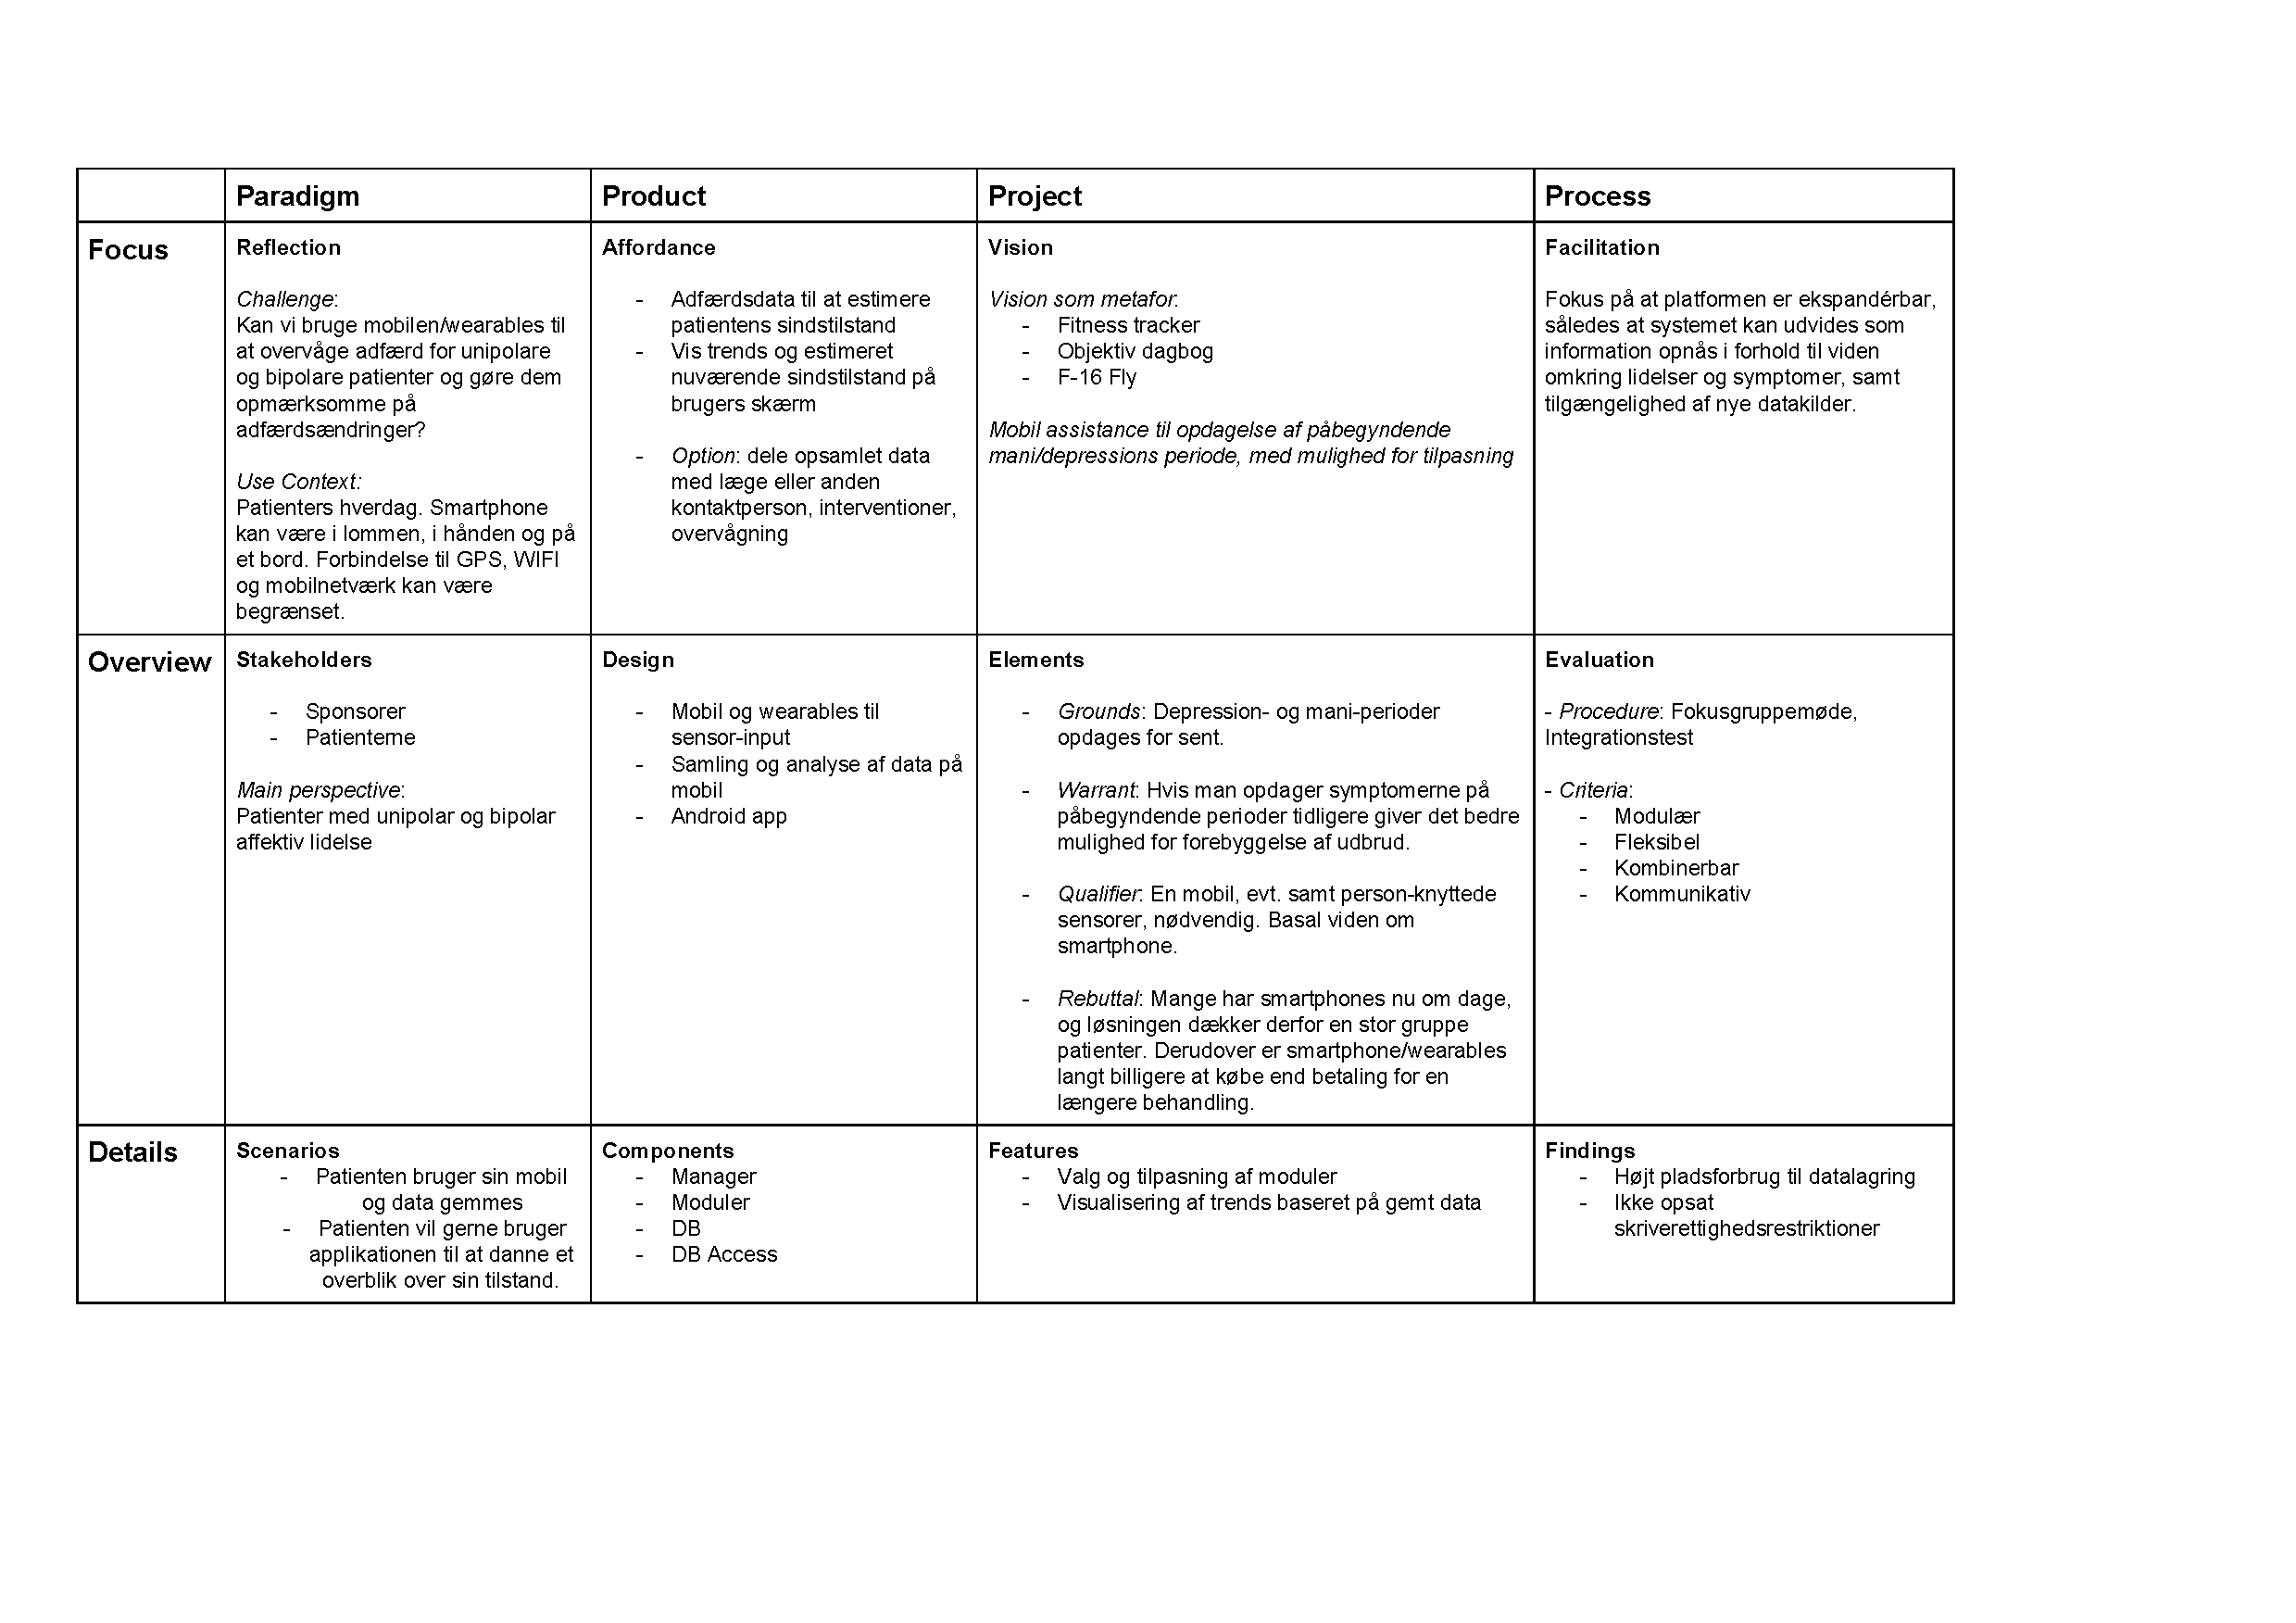
\includegraphics[scale = 0.65,trim = 1cm 3cm 6cm 2cm, angle = 90, clip]{KonfigurationTabel-frarapport.pdf}
\caption{En konfigurationstabel af systemet.}
\label{tab:konfigurationsTabel}
\end{figure}

\section{Vision}
\stefan{jeg tror dette afsnit skal væk, det er overlap med \ref{projectvisionrepr}}
Vores vision for projektet repræsenteres ved hjælp af Metaphor, specifikt formuleres det ved hjælp af tre metaforer.
Disse metaforer er \textit{Objektiv dagbog}, \textit{Fitness tracker} og \textit{F16 fly}.
At formulere vores vision som en metafor lader os koncist specificere hvad der er nøgleaspekterne af produktet.

Den objektive dagbog danner tanken om en dagbog baseret på objektive datakilder, hvilket svarer til sensor data, brugsdata etc.
Alt sammen data der kan indsamles uden brugerinteraktion.

Fitness trackeren som metafor planter tanken om en applikation, der løbende evaluerer ens præstationsevne, hvilket kan oversættes til mentalt helbred.

F16 fly metaforen henvender sig til platforms designet, der er tiltænkt at være en meget modulær og kraftig platform, ligesom det er tilfældet med F16 flyet hvor man kan hægte en lang række komponenter på alt efter hvad der er brug for i den pågældende situation.



\section{Use Cases}
I \citet[Afsnit 13.3, s83, nederst]{art:essence} beskrives fire forskellige elementer der skal overvejes i forbindelse med kreationen af brugs scenarier.
Disse overvejelser skal ligge på stakeholders, kontekst, teknologi og problemer.
Stakeholders er hvem scenariet har effekt på, kontekst er i hvilke omgivelser scenariet finder sted og hvilken effekt det har, teknologi er hvilke teknologiske muligheder der allerede eksisterer, problemer er hvad alt hvad der kunne give grundlag for en ændring.

For de scenarier der præsenteres er kontekst og stakeholders vurderet til at være de samme, selvom der i \citet[Afsnit 13.3, s83, nederst]{art:essence} siges at de sagtens kan variere fra et scenarie til et andet.

\subsection{Kontekst}
Konteksten som applikationen skal kunne bruges i er meget bred, da den omfatter hele patientens hverdag og alle tænkelige lokationer en patient kan opholde sig i løbet af sådan en dag.
Der skal derfor tages højde for at forbindelse til GPS, WIFI og mobilnetværk ikke altid er tilgængelige.
Da applikationen skal logge data om patientens færden skal der sikres håndtering af en række forskellige tilfælde angående brug og placering af smartphone.
Smartphonen kan eksempelvis være i lommen, i hånden, på et bord eller i lommen på en jakke der hænger i entréen.
Dette betyder at konteksten kan variere fra ude i en skov uden dataforbindelse til patientens arbejde.

\subsection{Stakeholders}
I dette projekt er patienterne den vigtigste \textit{stakeholder}, da det er patienterne, der skal bruge systemet i hverdagen.
Systemet skal derfor udvikles på patienternes præmisser.
I dette projekt er det specifikt patienter med unipolar eller bipolar affektiv lidelse vi beskæftiger os med.

Der er et antal sponsorer tilknyttet projektet, med dette menes folk der har interesse i projektet uden at være direkte stakeholders, da de ikke er tiltænkt at skulle bruge systemet.
Morten Aagaard har både erfaring inden for datalogi og psykologi og kan agere bindeled mellem de to discipliner.
Janne Vedel Rasmussen og Jørgen Aagaard arbejder inden for psykologifaget og kan derfor bidrage med fagrelevant information.
De har derudover en interesse i at få udviklet værktøjer der kan bidrage til deres arbejde.

\subsection{Scenarios}
Her undersøges hvordan \textit{the Challenge} bliver set fra brugerens perspektiv.
Teknikker til denne undersøgelse inkluderer at udforske systemets problemdomæne ved hjælp af \textit{Use scenarios}.

\paragraph{Use scenarios}
\textit{Use scenarios} bruges til at udforske ideer og muligheder i forhold til brugerens brug af systemet.

\subparagraph{Scenarier:}
\begin{itemize}
	\item Patienten bevæger sig rundt i sin hverdag med smartphonen i lommen. 
	\begin{itemize}
		\item Data logges i systemet, som gemmes til senere analyse.
	\end{itemize}
	
	\item Patienten vil gerne have applikationen til at fortælle hvordan den vurderer hans tilstand.
	\begin{itemize}
		\item Applikationen viser at patienten udviser normal adfærd.
		\item Applikationen viser at patientens stemningsleje er lavere end normalt.
		Patienten konsulterer sin liste af lystbetonede aktiviteter og udfører en af disse.
		\item Applikationen viser at patientens stemningsleje er lavere end normalt.
		Patienten foretager sig intet og tilstanden fortsætter med at forværres.
	\end{itemize}
\end{itemize}
Der er også et enkelt ekstra scenarie hvor der er en kontaktperson som stakeholder.
Den eksterne kontaktperson kan være mange ting, fx en patients kone, en nær ven eller en læge.
\begin{itemize}
	\item Applikationen registrerer fald af tilstand gennem en længere periode
	\begin{itemize}
		\item Tilstanden rammer et kritisk niveau og kontaktperson kontaktes
	\end{itemize}
\end{itemize}

\subsection{Technologies}
Dette koncept er beskrevet i \citep[Afsnit 13.3, s83, nederst]{art:essence}
Den smartphone systemet kører på kan bruges til at assistere i at fortælle patienten er tilstanden er blevet, eksempelvis i form af vibration eller afspille en lyd.
\lars{ARGH satan, ved ikke om dette kan blive til noget fornuftigt.}

\subsection{Problems}
Af potentielle problemer der kunne være er, at smartphone for ofte befinder sig i en kontekst hvor den indsamlede data ikke kan bruges, hvilket vil kræve en ændring, muligvis i form af en måde at registrere kontekst så data kan filtreres i når det kan bruges og når det ikke kan bruges.
Et andet problem der kan opstå er, at det ser ud som om smartphone er på en person, men det er bare ikke den patient det er meningen der skal analyseres på.
Dette problem kræver en form for persongenkendelse så data fra andre personer kan filtreres fra.

For det andet sæt af scenarier hvor patienten går ind og ser sin tilstand, er der også noget der kan kræve ændring.
Den første er at patienten ikke bruger det ofte nok og derfor ikke bliver informeret om sin tilstandsændring tids nok til at det rent faktisk betyder noget.

I det sidste scenarie, for at bestemme et kritisk niveau skal baseres ud fra individet, desuden kan det for nogen individer kræve øjeblikkelig indlæggelse.
Hvis en sådan patient registreres i kritisk tilstand, er det ikke nok bare at kontakte en kontaktperson, men burde nok nærmere tilkalde en ambulance.
Der er også den risiko at det at kontakte en kontaktperson bliver vurderet som problematisk i forhold til patient empowerment konceptet som dette gerne skulle hjælpe med. 

 %A description of use context and selected use scenarios (see Essence-book Chapter 13).
\section{Diskussion af implementation af hovedscenarier}
Udtrækning af klasser af tilstande fra use cases nævnes i \citet[Afsnit 14.4, s94]{art:essence} som en metode til at finde features der skal arbejdes på i projektet.

Det at gå ind i ens use cases giver et fornuftigt fundament for de vanskeligere overvejelser i ens design proces.

Ud fra de use cases, der tidligere er præsenteret findes følgende essentielle tilstandsklassificerings problemer:
\begin{enumerate}
\item På korrekt person? \label{korrekt}
\item Tilstands ændring? \label{tilstand}
\item Kritisk tilstand? \label{kritisk}
\end{enumerate}

Til \textbf{problemstilling \ref{korrekt}} er der flere potentielle løsninger af varierende kompleksitet.
En mulighed er at bruge en fingeraftrykslæser og så med jævne mellemrum bede bæreren af smartphonen om en scanning.
Dette vil begrænse grupperingen til intervaller, og eftersom man ikke kan scanne patienten hele tiden, vil det størrelsen af intervallet have en effekt på præcisionen af forudsigelsen.
En anden mulighed er at bruge data telefonen indsamler til at bestemme hvilken person der bruger telefonen.
En mulighed kan være at analysere personers gangart ud fra accelerometer data og derved identificer bæreren af telefonen.

\textbf{Problemstilling \ref{tilstand}} kræver indsamling af meget data fra mange forskellige kilder for at have et grundlag for en vurdering af patientens tilstand.
Hvilke datakilder der skal benyttes kan variere meget fra individ til individ.
Et individ kunne for eksempel have brug for at få set på sit bevægelsesmønster og på sin sociale adfærd, hvor et andet kunne have brug for at få analyseret på søvn og på hvor meget han har forladt sit hjem.
At kunne se på disse er udfordrende i sig selv, da man for hver af disse skal finde ud af hvilke datakilder man har til rådighed, der kan give en fornuftig information om disse, og derefter skal man finde ud af hvordan man ud fra data kan lave en vurdering af det givne kriterie.

\textbf{Problemstilling \ref{kritisk}} afhænger af at man kan vurdere om en tilstand er kritisk.
Det er også nødvendigt at vurdere hvad man rent faktisk skal gøre når en patient vurderes i en kritisk tilstand.
En mulighed er at konstruere en model over patientens tilstand og ud fra det vurdere hvor langt det er acceptabelt at patienten afviger fra denne baseline.
Når patientens tilstand vurderes som kritisk kan man kontakte lægen eller nærmeste pårørende
Hvorefter de kan tage en beslutning om hvad der skal ske. % A discussion of how to implement support for key use scenarios (see Essence-book Chapter 14).
\section{Representation of Project Vision}
Der findes flere måder at præsentere sin vision på. 
I \citet[Kapitel 24 - Representation]{art:essence} præsenteres fire repræsentationer, \textit{Metafor}, \textit{Ikon}, \textit{Prototype} og \textit{Proposition}.

Vi har valgt at repræsentere vores vision ved hjælp af metaforer, da denne repræsentation er abstrakt og giver meget plads til fortolkning.
Metafor-repræsentationen giver en beskrivelse af hvad fokusområdet er, uden at afgrænse fra at se på andre retninger.

De tre metaforer vi har benyttet er \textit{Objektiv dagbog}, \textit{Fitness tracker} og \textit{F-16 fly}.

\textbf{Den objektive dagbog} danner tanken om en dagbog baseret på objektive datakilder, hvilket svarer til sensor data, brugsdata etc.
Alt sammen data, der kan indsamles uden direkte brugerinteraktion, altså uden at brugeren bevidst gør ting der har effekt på den indsamlet data.

\textbf{Fitness trackeren} som metafor planter tanken om en applikation der løbende evaluerer ens præstationsevne, hvilket kan oversættes til helbred, herunder mentalt helbred.

\textbf{F-16 fly}\label{vision::fly} metaforen henvender sig til designet af platformen, der er tiltænkt at være modulær, ligesom det er tilfældet med F-16 flyet, hvor man kan hægte en lang række komponenter på alt efter hvad der er brug for i den pågældende situation.
Her har vi varierende symptomer, hvilket kræver at indsamling og analyse af data kan skifte efter behov.
 % A representation of your Project Vision and (if relevant) Prospect Research (see Essence-book Chapter 15).
\section{Kriterier}\label{firstsubseckriterier}
Her bliver de vigtigste kriterier præsenteret, som skal opfyldes for at kunne kalde projektet en succes.
Disse kriterier er de samme som kan findes i konfigurationstabellen (\cref{tab:konfigurationsTabel}).
Kriterierne opstilles til at kunne evaluere ens løsning.

\begin{description}[style=nextline]
	\item[Modulær] 
	Da individer kan have forskellige symptomer skal det være muligt at tilføje og fjerne datakilder, samt analyser af disse, så den enkelte patient får den bedst mulige behandling.
	\item[Fleksibel]
	Det skal være nemt at modificere funktionalitet til platformen, da platformen skal kunne tilpasses til individet.
	\item[Kombinerbar] Eftersom vi prioriterer modulærbarhed skal ansvarsområder være lette at separere så indhentede data kan bruges på tværs af systemet.
	\item[Kommunikativ] Data skal være tilgængeligt på tværs af systemet, men skal samtidig være beskyttet mod at blive redigeret af uvedkommende.
\end{description}

Kriterierne opstilles til at evaluere ens løsning.
Resultaterne af denne evaluering  noteres i ``findings'' og danner grundlag for den næste konfigurationstabel.
Der kan læses om et eksempel på brug af kriterier i \citet[Kapitel 2.2, 2.3, 2.4 og 2.5 side 16--21]{art:essence}.

\subsection{Evaluering af kriterier}
\begin{description}[style=nextline]
	\item[Modulær]
	Hele arkitekturen er opbygget af en manager applikation og en række separate moduler, som kan bruges i manageren.
	Dette understøttes af den fælles datagrænseflade i form af DBAccess og moduldefinitionerne.  
	Det er muligt at specificere at man er afhængig af blot et modul eller af en mængde af disse.
	Eksempelvis er det muligt for et analysemodul at afhænge af et accelerationsmodul.
	
	Som et eksisterende eksempel på at moduler nemt kan tilføjes og bruges af manageren er udviklede moduler, beskrevet i \citet{misc:soevnrapp} og \citet{misc:surveyrapp}.
	Disse eksempler viser også hvorledes det er muligt at udvikle moduler, der afhænger af data fra andre moduler.
	
	\item[Fleksibilitet]
	Til at sikre at platformen er fleksibel i forhold til patienten, hvor de har kontrol over hvilke moduler, der kan køre, tilbydes dette i form af en indstillingsmenu.
	Endvidere har patienten også kontrol over hvilke moduler, der er installeret på deres smartphone, idet hvert modul er en separat applikation på deres smartphone, som de sagtens kan afinstallere hvis ønsket.
	
	\item[Kombinerbar]
	Data indsamlet fra diverse moduler kan benyttes af andre moduler, eksempelvis analysemoduler.
	Et klart eksempel på dette kan læses i \citet{misc:soevnrapp}, hvor data fra et søvnestimeringsmodul for acceleration og et modul for amplitude kombineres i et samlet søvnestimeringsmodul.
	
	\item[Kommunikativ]
	Det kommunikative kriterie er understøttet i den grad at data nemt kan kommunikeres til relevante moduler.
	Dog er sikkerhedskriteriet for denne kommunikation \textit{ikke} på plads.
	Derudover er der ikke opsat skriverettighedsrestriktioner, og således er der altså et kriterie der ikke er blevet opfyldt og skal arbejdes videre med før man kan konkludere at en tilpas færdig platform er udviklet.
\end{description}

Ud fra denne evaluering har vi en finding der gå på manglende skriverettighedsrestriktioner.
Desuden kan vi erfare at kriterierne om modularitet, fleksibilitet og kombinerbarhed er opfyldt.
 % Key criteria for evaluations in your project plus one or more examples of evaluations  (see Essence-book Chapter 16).
\section{Vision Scenarios}
Hele dette afsnit bygger på \citet[Sektion 17.1]{art:essence}, hvor der foreslås en teknik kaldet \textit{vision scenarios} til at nærmere bestemme fokus for et projekt.
For at styre dette projekt i den rigtige retning er der blevet lavet vision scenarios som hjælper med dette.
Til at lave vision scenarios er det nødvendigt at tildele roller til de forskellige personer der er med i projektet.
Rollerne der skal udleves er Child \citep[Kapitel 18]{art:essence}, Challenger \citep[Kapitel 19]{art:essence}, Responder \citep[Kapitel 20]{art:essence} og Anchor \citep[Kapitel 21]{art:essence}.

\subsection{Bestemmelse af retning}
For at hjælpe med at bestemme retning for projektet, hvor der var flere interessante bud, opsættes \textit{vision scenarios}.
Her sættes flere modsætninger overfor hinanden, hvor hver modsætningspar kan føre projektet i to forskellige retninger.
I vores tilfælde fandt vi seks forskellige modsætninger vi syntes kunne være interessante at kigge på:
\begin{itemize}
	\item Én Lidelse kontra Flere lidelser
	\item Personligt kontra Delt med læge
	\item Udregning i skyen kontra Lokal udregning
	\item Opbevaring i skyen kontra Lokal opbevaring
	\item Bruger input kontra Sensor input
	\item Interventioner kontra Patient empowerment
\end{itemize}

Ud af disse seks modsætningspar blev der udvalgt de 2 vurderet mest relevante, hvilket blev gjort på demokratisk vis.
Dette førte til en 2-dimensioneal sammenligning, hvor på den ene akse er der opsat \textit{Bruger input} gående mod \textit{Sensor input} og på den anden akse \textit{Interventioner} gående mod \textit{Patient empowerment}.
Derefter anskues alle 4 kombinationer af begreber med de 4 forskellige roller.

\newcommand{\coord}[8]{
\begin{center}
\begin{tikzpicture}
[
    scale=5,
    axis/.style={very thick, <->, >=stealth'},
    important line/.style={thick},
    dashed line/.style={dashed, thin},
    pile/.style={thick, ->, >=stealth', shorten <=2pt, shorten
    >=2pt},
    every node/.style={color=black}
    ]
    \tikzstyle{every node}=[font=\small]
    \draw[axis] (-1,0) node(xline)[below]{#1}  -- (1,0) node(xline)[below]{#2};
    \draw[axis] (0,-1) node(yline)[right]{#4} -- (0,1) node(yline)[left]{#3};
    \node[draw=none,align=center,text width=3cm] at (-0.5,0.5){#5};
    \node[draw=none,align=center,text width=3cm] at (0.5,0.5){#6};
    \node[draw=none,align=center,text width=3cm] at (0.5,-0.5){#7};
    \node[draw=none,align=center,text width=3cm] at (-0.5,-0.5){#8};
\end{tikzpicture}
\end{center}
}


\subsection{Child}
Dette er den eneste rolle alle i projektet kan have på vilkårlige tidspunkter.
Det er også denne rolle der sørger for at der kommer kreative idéer og er helt central for hvordan idéer bliver lavet i samarbejde mellem udviklere og kunder.

\coord
  {Bruger Input}
  {Sensor Input}
  {Interventioner}
  {Patient Empowerment}
  {Brug bruger input til at opdage påbegyndende forværring i tilstand og oplys patienten om dette.}
  {Brug objektive datakilder til at opdage påbegyndende forværring i tilstand og oplys patienten om dette.}
  {Brug objektive datakilder til at samle information om patientens nuværende tilstand og gøre dette tilgængeligt for patienten.}
  {Brug bruger input til at samle information om patientens nuværende tilstand og gøre dette tilgængeligt for patienten.}

\subsection{Challenger}
Det er den der snakker på vegne af \textit{stakeholders}.
Det er også ud fra denne rolle der gives opgaver, prioriteres opgaver og accepteres løsninger.
Derudover skal dem som har rollen være inspirerende i den forstand at de skal kunne få udviklere til at se flere mulige løsninger. 
Challenger bruges på denne måde til at sørge for at den løsning der vælges er den rigtige løsning, samt om det er den bedste løsning der kan blive lavet.

\coord
  {Bruger Input}
  {Sensor Input}
  {Interventioner}
  {Patient Empowerment}
  {Ud fra bruger input registeres ændring i adfærd til at foreslå lystbetonede aktiviteter.}
  {Ud fra objektive datakilder registeres ændring i adfærd til at foreslå lystbetonede aktiviteter.}
  {Visualisere sensor input så brugeren kan blive opmærksom på sine ændringer i adfærd.}
  {Visualisere bruger input så brugeren kan blive opmærksom på sine ændringer i stemningsleje.}

\subsection{Responder}
Responders opgaver består i at lave mulige løsninger om til færdige løsninger og at løse de forskellige opgaver der bliver givet.
Denne rolle består af udviklerne og det er derfor denne rolle der står for prototypes og alle de tekniske løsninger.
Responder rollen bruges til at se om man har udnyttet det fulde potentiale af projektet.
Her er der tale om man bruger de rigtige komponenter, men også om man bruger disse komponenter så meget som man overhovedet kan. 

\coord
  {Bruger Input}
  {Sensor Input}
  {Interventioner}
  {Patient Empowerment}
  {Tilpasset dagbog baseret på tidligere dagbogsindlæg.
    Struktureret så data kan analyseres og sammenlignes og derudfra foretage interventioner.}
  {Brug sensor data til at foreslå interventioner til brugeren baseret på trends, fx. gang, søvn eller social aktivitet.}
  {Visualisere sensor data så patienten kan vurdere sin tilstand.}
  {Elektronisk dagbog med løs tekst.}

\subsection{Anchor}
Anchor er den der skal beskytte udviklerne fra at blive forstyrret og glemme hvad fokus er.
Dernæst er det også denne rolle der sørger for at planlægge specielle events, såsom sprint planning.
Anchors rolle er at sørge for at alle stakeholders er tilfredse med det der bliver udviklet.
Derudover er det også deres opgave at beskrive de fordele og ulemper der er ved de forskellige idéer, visioner, prototyper og strategier.

\coord
  {Bruger Input}
  {Sensor Input}
  {Interventioner}
  {Patient Empowerment}
  {Hvordan kan det afgøres om man skal foretage interventioner?
    Hvordan kan dagbogindslag sammenlignes?
    Hvordan vælges hvilken intervention?}
  {Hvordan kan det afgøres om der skal foretages en intervention?
    Hvordan identificere man trends og ændring i adfærd?
    Hvordan vælges hvilken intervention?}
  {Hvordan kan man visualisere meget data?
    Hvordan kan data aggregeres?}
  {Hvordan får brugeren overblik over sin dagbog?}
 % Characterization of your project using Vision Scenarios  (see Essence-book Part 4):
\section{Example of Idea Maturation}

Der er mange ændringer, vi snakker om disse:

Evaluation

Stakeholders

Features

\todo[inline]{skriv ting}

\begin{figure}
	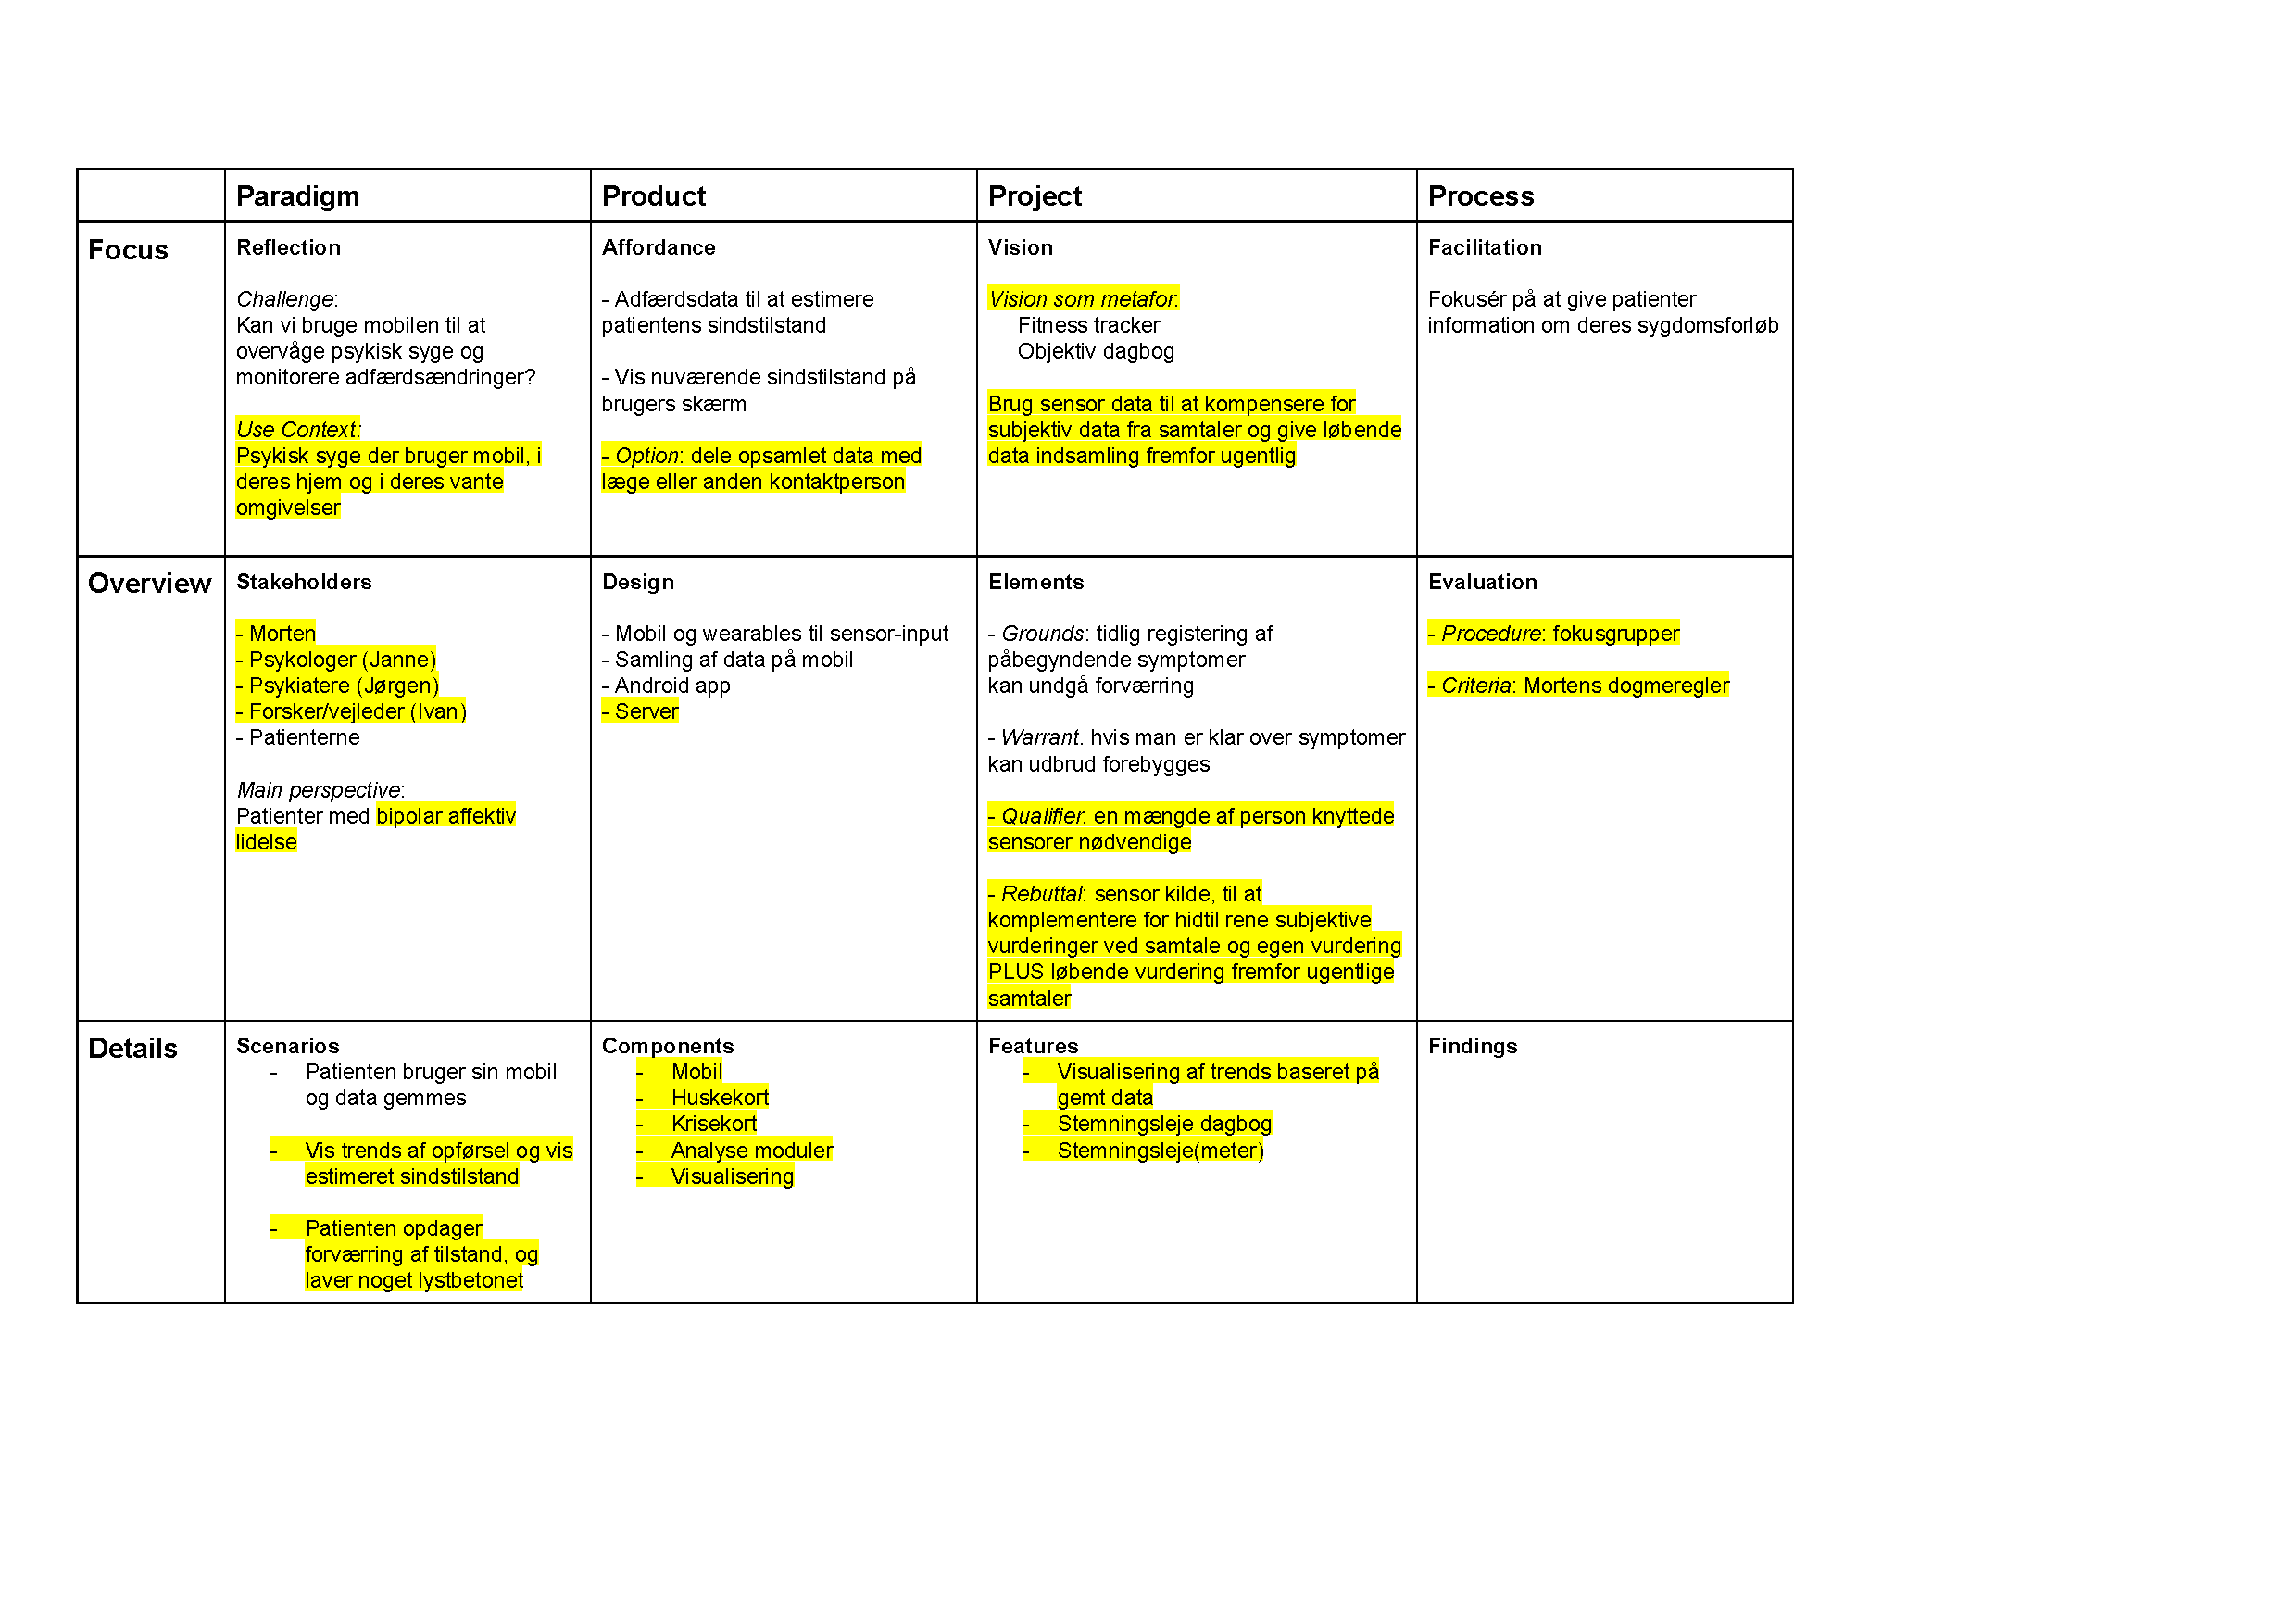
\includegraphics[scale = 0.65,trim = 1cm 3cm 6cm 2cm, angle = 90, clip]{tidlig-konfigurationstabel.pdf}
	\caption{En konfigurationstabel på et tidligt stadie af udviklingen}
	\label{tab:tidligKonfigurationsTabel}
\end{figure} % Give an example of idea maturation
\section{Theoretical Evaluation}

\subsection{Software team dynamik}
Om et software team er innovativt afhænger af en mængde faktorer som teamet sjældent har kontrol over.
Disse faktorer varierer fra omgivelserne de sidder i, til de krav der bliver stillet fra deres overordnede.
Et udvalg af disse faktorer vil i dette blive beskrevet (taget fra \citet[s.~81-82]{book:softwareinnovation}), hvorefter vi vil vurdere deres indflydelse på vores projekt.

\begin{description}[style=nextline]
	\item[Tidspres] Når et team arbejder under tidspres forhindrer det at teamet bruger tid på refleksion, hvilket udelukker at der bruges tid på at udforske og eksperimentere med mulige løsninger.
	\item[Stress] Stress har både fysiologiske og psykologiske effekt på produktiviteten. Når et team er stresset forværres kommunikationen internt hvilket har en negativ effekt på produktet.
	\item[Ressource mangel] Mangel på ressourcer tvinger teamet til de vante arbejdsgange, i stedet for eksperimenterende tilgange til problemer.
	\item[Strengt definerede arbejdsgange] Hvis teamet er tvunget til et sæt af prædefinerede arbejdsgange fra deres overordnede besværliggør det refleksion.
	\item[Bureaukrati] Overdokumentation af teamets arbejde tvinger holdet til at følge de definerede processer 
	\item[Rutinearbejde] For meget rutinearbejde får teamets medlemmer til ikke at se opgaverne i et alternativt perspektiv.
	\item[Dårlig projektstyring] Autoritære projektstyringsstile har en negativ indflydelse på innovative karakteristikker som dialog.
\end{description}

I det følgende vil det blive beskrevet 

\paragraph{Semester}
Da vi er dikterede af studieordningens indhold er der nogle forhold som vi ikke selv er herre over.
For det første løber semestret over en prædefineret periode hvilket introducerer et \textbf{tidspres}.
Studieordningen kræver også at arbejdet bliver dokumenteret i en rapport hvilket er en blanding af \textbf{bureaukrati} og \textbf{strengt definerede arbejdsgange}.

\paragraph{Vejleder}
En barriere der ikke har været i projektet er \textbf{ressource mangel}, da vores vejleder fra starten har bidraget til projektet både med indsigt og med ressourcer som smartphone og smartwatch.

\paragraph{Teamet}
Teamet har i til dels været tilbøjelig til \textbf{rutinearbejde} i forhold til strukturen i projektet.
Tasks defineres, kodes og dokumenteres uden videre eftertanke om, hvorvidt vi er på vej i den rigtige retning.
\textbf{Dårlig projektstyring} er i kilden defineret ud fra autoritære projektstyringsstile.
I vores projekt har det omvendte været problemet, der har ikke været én projektleder, men i stedet har vi alle haft en del af lederrollen.
Dette har betydet at ledelsen har været løs og uden retning.

\subsubsection{Improvisering}
Improvisering er en stor del af software innovation som \citet[side 56]{book:softwareinnovation} siger: \textit{Improvisation and bricolage flesh out the skeleton, whatever the underlying process. Developing technically exploratory software involves manoeuvring in uncharted waters, where development platforms are uncertain and untried, so it is unlikely that generic process models or formal development methods can provide enough support for the developer.}
Derfor har det selvfølgelig også været en stor del af vores proces, og denne improvisering har taget forskellige former.
Som \citet[side 56]{book:softwareinnovation} siger: \textit{In a development situation, improvisation often takes the form "let's try this...:" a customer meeting, a programming technique, a diagramming technique, a different hardware component.}
Af disse former har vi mødt med interesserede personer og patienter med psykiske lidelse for at få deres perspektiv og deres idéer om platformen og hvad der kan gøres med de data kilder der er tilgængelige. 
Ydermere har vi brugt brainstorming, idet vi så på de forskellige sensorer og kom med idéer om hvad de kunne bruges til for at få kontaktpersonernes holdninger om dette.
På samme tid har vi også brugt diagram teknikker, til at opklare hvordan den tiltænkte arkitektur skulle se ud.
Dette er blevet brugt til at lave flere versioner af arkitekturen og af disse er der blevet foretaget et valg. % Theoretical evaluation. Compare your work with some of the theories that are referred to in the course literature. The evaluation should not be value judgment-based, but should seek to relate your work to the theories and principles that the course draws from. You might like to focus on 

\bibliographystyle{unsrtnat}
\bibliography{bib}
\label{bib:mybiblio}

\appendix
\end{document}
